\documentclass{beamer}
\mode<presentation>
\setbeameroption{show notes}

\usepackage{listings} % добавление листингов из исходников
\usepackage{IEEEtrantools} % для создания многострочных математических формул

\usepackage[utf8]{inputenc}
\usepackage[russian]{babel}
\usepackage{pdfpages}
\usepackage{graphicx}
\usepackage{tikz}
\usepackage{xcolor}
\usepackage{multirow}

\usepackage{amsfonts}

\setbeamertemplate{navigation symbols}{
	\insertframenavigationsymbol
	\raisebox{0.07cm}[0pt][0pt]{
    \insertframenumber/\inserttotalframenumber}
}

\setbeamertemplate{frametitle}[default][center]


\title{Local Alignment Kernels for Biological Sequences}
\author{Свичкарев Анатолий}

% поля титульного слайда
\institute{Санкт-Петербургский Государственный Политехнический Университет\\
    Петра Великого\\
    \vspace{0.7cm}
    Преподаватель:  к.н. Н.О. Кадырова\\
    \vspace{0.7cm}
}
\date{\today}

\begin{document}

% титульный слайд
\begin{frame}
\titlepage
\end{frame}

\begin{frame}
\frametitle{Вступление}
\begin{itemize}
    \item Локальное выравнивание
    \item Алгоритм Смита-Ватермана
    \item Свёртка ядер
    \item Построение ядра локального выравнивания
    \item Эксперимент
    \item Выводы
\end{itemize}
\end{frame}

\begin{frame}
\frametitle{Локальное выравнивание последовательностей\\
Обозначения}
Выравнивание с пробелами:
\begin{equation*}
    \pi = ((\pi_1(1), \dots, \pi_1(p)),(\pi_2(1), \dots, \pi_2(p)))
    \in \mathbb{N}^{2p}
\end{equation*}

Пример: x = GAATCCG и y = GATTGC
\begin{equation*}
    \pi = ((1,2,4,6),(1,3,4,5))
\end{equation*}
\centerline{G-AATCCG-}\\
\centerline{GAT-T-G-C}
\end{frame}

\begin{frame}
\frametitle{Локальное выравнивание последовательностей\\
Алгоритм Смита-Ватермана}
Счёт локального выравнивания:
\begin{IEEEeqnarray*}{rCl}
    S_{S,g}(\pi)
    & = & \sum_{i=1}^{|\pi|}S(x_{\pi_1(i)}, y_{\pi_2(i)}) - \\
    - && \sum_{i=1}^{|\pi|-1}(g(\pi_1(i+1) - \pi_1(i))
    + g(\pi_2(i+1) - \pi_2(i)))
\end{IEEEeqnarray*}
Счёт Смита-Ватермана (SW):
\begin{equation*}
    SW_{S,g}(x, y) = \max_{\pi \in \Pi(x, y)} S_{S, g}(\pi)
\end{equation*}
\end{frame}


\begin{frame}
\frametitle{Подходит ли SW в качестве ядра?}
Напомим определение допустимого ядра:
\begin{itemize}
    \item симметрия:
    \begin{equation*}
        k(x, y) = k(y, x)
    \end{equation*}

    \item положительная полуопределённость:
    \begin{equation*}
        \forall n \in \mathbb{N},
        \forall (x_1, \dots, x_n, \alpha_1, \dots, \alpha_n)
            \in \chi^n \times \mathbb{R}^n:
    \end{equation*}
    \begin{equation*}
        \sum^n_{i, j = 1} \alpha_i \alpha_j k(x_i, x_j) \geq 0
    \end{equation*}
\end{itemize}
будем называть такие ядра \textit{\textbf{строковыми}}.

\bigskip
\textbf{Проблема:}\\
SW симметрично,\\но не всегда положительно полуопределено.

\bigskip
Авторы решили разобраться...
\end{frame}

\begin{frame}
\frametitle{Свёртка ядер}
Определение:

\begin{equation*}
    \sqsupset k_1, k_2 \mid k_i: \chi \times \chi \to \mathbb{R}.
\end{equation*}
Свёрткой $k_1$ и $k_2$
назовём $k_1 \star k_2$:
\begin{equation*}
    k_1 \star k_2(x, y)
    = \sum_{x_1 x_2 = x, y_1 y_2 = y} k_1(x_1, y_1) k_2(x_2, y_2)
\end{equation*}

\bigskip
Теорема:

Свёртка двух строковых ядер --- строковое ядро.
\end{frame}

\begin{frame}
    \frametitle{Построение ядра локального выравнивания (LA)}
    Сконструируем новое строковое ядро из трёх простых ядер.
    \bigskip

    Будем использовать:
    \begin{equation*}
        \forall (x, y) \in \chi^2
    \end{equation*}

    \begin{itemize}
        \item Края:
            \begin{equation*}
                k_0(x, y) = 1
            \end{equation*}

        \item Выровненные символы:
            \begin{equation*}
                k_\alpha^{(\beta)}(x, y) = \left\{ \,
                    \begin{IEEEeqnarraybox}[][c]{l?s}
                        \IEEEstrut
                        0 & если $|x| \ne 1$ или $|y| \ne 1$, \\
                        exp[\beta S(x, y)] & иначе.
                        \IEEEstrut
                    \end{IEEEeqnarraybox}
                    \right.
                    \label{eq:example_left_right1}
                \end{equation*}

        \item Пропуски:
            \begin{equation*}
                k_g^{(\beta)}(x, y) = exp[\beta (g(|x|) + g(|y|))]
            \end{equation*}
    \end{itemize}
\end{frame}

\begin{frame}
    \frametitle{Ядро локального выравнивания (LA)}
    Соединим всё вместе:
    \begin{equation*}
        k_{(n)}^{\beta} = k_0
            \star (k_\alpha^{(\beta)} \star k_g^{(\beta)})^{(n-1)}
            \star k_\alpha^{(\beta)} \star k_0
    \end{equation*}

    Сходство между $x$ и $y$
    с числом выровненных ровно $n$.
    \bigskip

    Для $n = 0: k_{(0)}^{\beta} = k_0$.
    \bigskip

    \textbf{LA ядро:}
    \begin{equation*}
        k_{LA}^{\beta} = \sum_{i=0}^{\infty}k_{(i)}^{\beta}
    \end{equation*}
\end{frame}

\begin{frame}
\frametitle{Связь LA ядра с SW}
Выражение LA ядра через счёт локального выравнивания:
\begin{equation*}
    \forall (x, y) \in \chi^2
\end{equation*}
\begin{equation*}
    k_{LA}^{\beta}(x, y) = \sum_{\pi \in \Pi(x, y)}exp(\beta S_{S, g}(x, y, \pi))
\end{equation*}
\bigskip

Счёт SW соотносится с LA ядром следующим выражением:
\begin{equation*}
    \lim_{\beta\to\infty} \frac{1}{\beta} \ln k_{LA}^{\beta}(x, y)
    = SW_{S,g}(x, y)
\end{equation*}

SW не является допустимым строковым ядром:
\begin{itemize}
    \item учитывает только лучшее выравнивание для измерения сходства;
    \item логарифм не всегда обеспечивает положительную полуопределённость.
\end{itemize}
\end{frame}

\begin{frame}
\frametitle{Вычисление LA ядра}
\begin{itemize}
    \item Модификация алгоритма Смита-Ватермана
    \item Конечный автомат
        \begin{figure}[h]
            \center{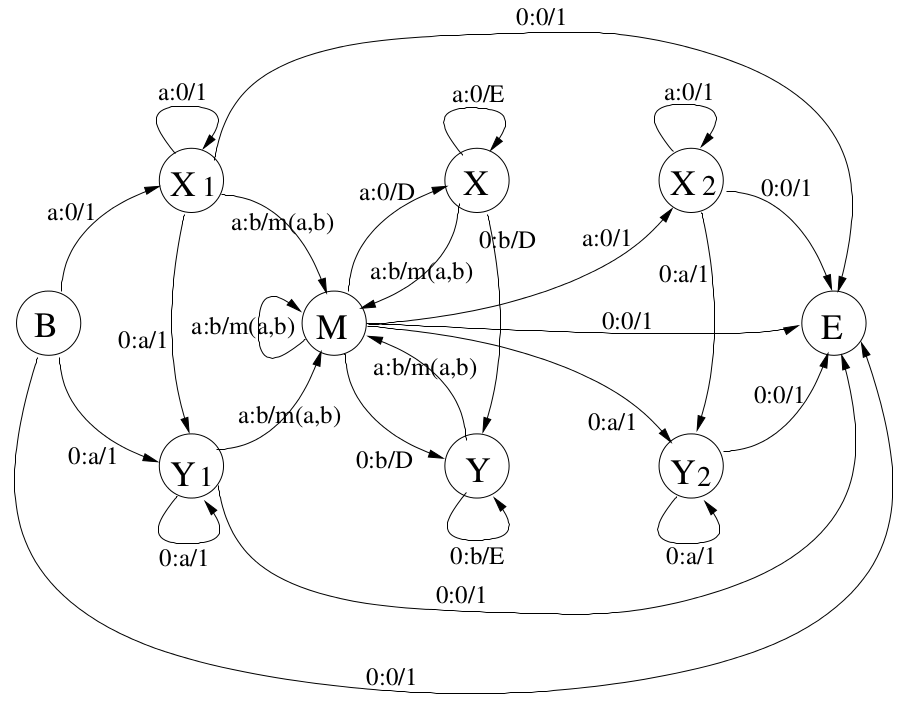
\includegraphics[width=\linewidth,height=7cm]{img/hmm}}
        \end{figure}
\end{itemize}
\end{frame}

\begin{frame}
\frametitle{Решение диагонального преобладания}
Нормализация, убирает диагональное преобладание с ростом $\beta$:
\begin{equation*}
    \widetilde{k}_{LA}^{\beta}(x, y)
    = \frac{1}{\beta} \ln k_{LA}^{\beta}(x, y)
\end{equation*}
Приведение к положительной полуопределённости:
\begin{itemize}
    \item Вычитание из диагонали
        наименьшего отрицательного собственного значения
        матрицы Грамма (LA-eig).
        \bigskip

    \item Эмпирическая ядерная таблица (LA-ekm):
    \begin{equation*}
        (\widetilde{k}_{LA}^{\beta}(x, x_1), \dots,
        \widetilde{k}_{LA}^{\beta}(x, x_n))
    \end{equation*}
    на обучающей выборке.

\end{itemize}
\end{frame}

\begin{frame}
\frametitle{Эксперимент}
\begin{columns}
\column{0.5\textwidth}
    Тестируемые методы:
    \begin{itemize}
        \item LA-eig
        \item LA-ekm
        \item Pairwise
        \item Mismatch
        \item Fisher
    \end{itemize}

\column{0.5\textwidth}
    Параметры выравнивания:
    \begin{itemize}
        \item белки
        \item BLOSUM62
        \item открытие пробела -11
        \item продолжение пробела -1
    \end{itemize}
\end{columns}
\bigskip

Задача классификации белковых доменов в суперсемейства:
\begin{itemize}
    \item 4352 белковых последовательности
    \item 54 семейства
    \item 10 положительных значений в обучающей выборке
    \item 5 положительных значений в тестовой выборке
    \item отрицательные получены
        смешиванием последовательностей в пропорции
\end{itemize}
\end{frame}

\begin{frame}
\frametitle{ROC-кривая}
\begin{columns}
\column{0.9\textwidth}
    \begin{figure}[h]
        \center{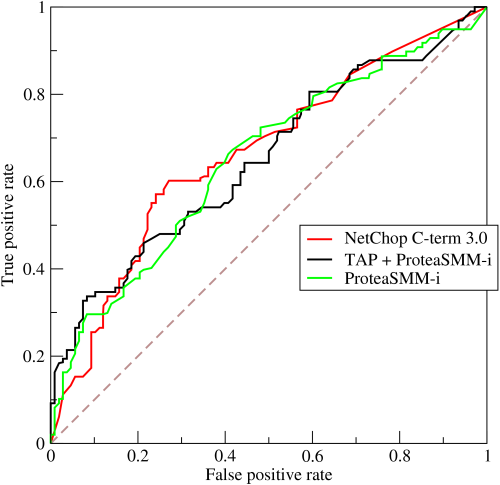
\includegraphics[width=\linewidth,height=7cm]{img/Roccurves}}
    \end{figure}

\column{0.3\textwidth}
    Критерии качества:
    \begin{itemize}
        \item Mean $ROC$
        \item Mean $ROC_{50}$
        \item Mean mRFP
    \end{itemize}
\end{columns}
\end{frame}

\begin{frame}
\frametitle{Результаты эксперимента}
    \begin{figure}[h]
        \center{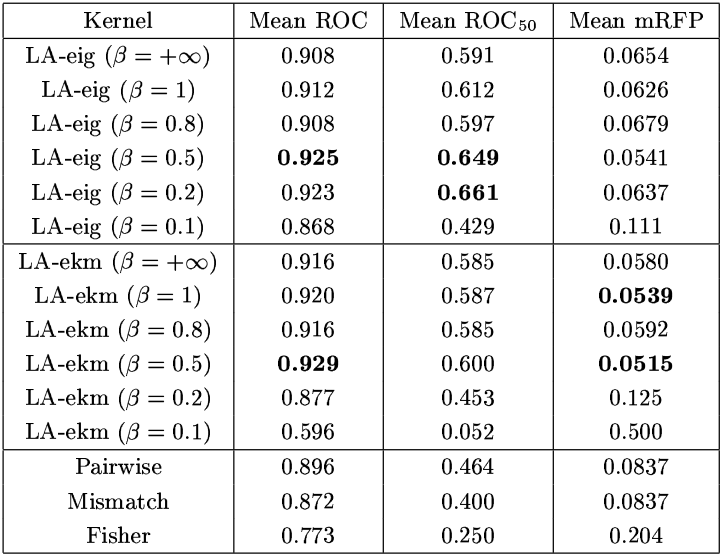
\includegraphics[width=\linewidth,height=7cm]{img/table}}
    \end{figure}
\end{frame}

\begin{frame}
\frametitle{Результаты эксперимента}
    \begin{figure}[h]
        \center{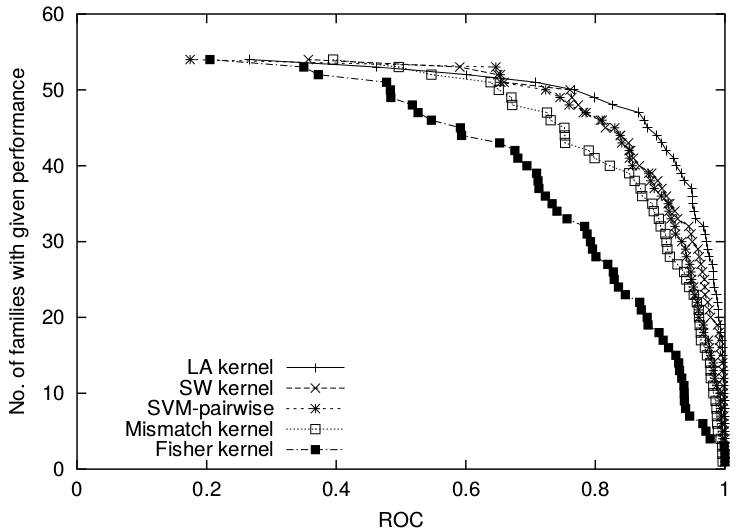
\includegraphics[width=\linewidth,height=7cm]{img/ROC}}
    \end{figure}
\end{frame}

\begin{frame}
\frametitle{Результаты эксперимента}
    \begin{figure}[h]
        \center{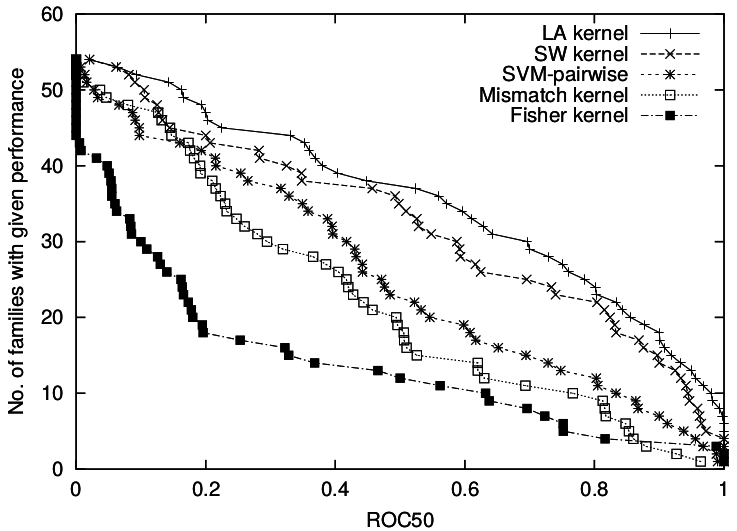
\includegraphics[width=\linewidth,height=7cm]{img/ROC50}}
    \end{figure}
\end{frame}

\begin{frame}
\frametitle{Результаты эксперимента}
    \begin{figure}[h]
        \center{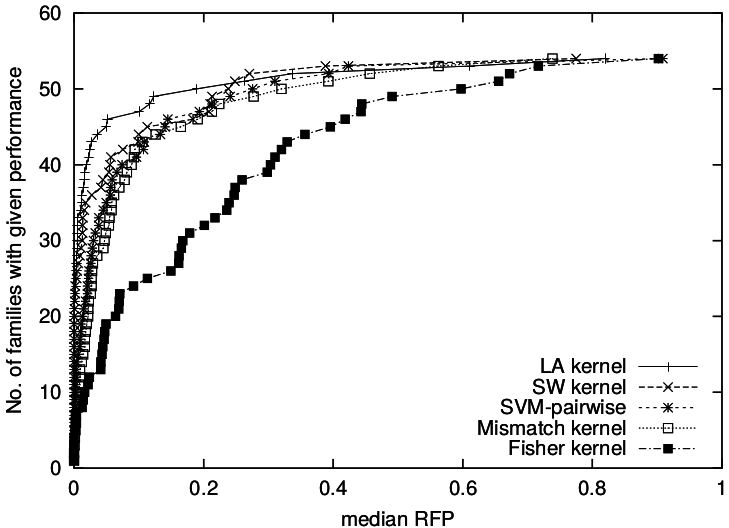
\includegraphics[width=\linewidth,height=7cm]{img/medianRFP}}
    \end{figure}
\end{frame}

\begin{frame}
\frametitle{Выводы}
\begin{itemize}
    \item Правильное применение SVM и SW даёт отличные результаты;
    \item Сумма всех локальных выравниваний превзошла SW;
    \item Важен компромис между скоростью и точностью;
    \item Не ясна зависимость $\beta$ от изменения
        штрафа за пропуск и матрицы замен;
    \item Не решена проблема зависимости ядра от длины последовательностей.
\end{itemize}
\end{frame}

\end{document}
